% pipeline_v6 (fig:pipeline, figure*): pipeline_v3 with a few key equations (user, 2026-11-02: "v3 is
% best. we can add a little equation to v3"); layout, pictures and labels of v3 unchanged otherwise.
% v3 (below) shows one keyframe update of the UAGS field in five stages, in
% the order the code runs them. Replaces pipeline_v2.tex (kept untouched), which had a formula
% block in each of its nine boxes: here each stage has a short title, one picture and at most one
% formula, in the style of RA-L / T-RO overview figures (E2-BKI, RA-L; ConvBKI, T-RO); the
% details are in the caption and in Sec. III. Thumbnails (validation scenes only) are those of
% v2, made by scripts/render_pipeline_thumbs.py: Replica office_0 mapping keyframe 825 (1, 4, 5);
% NeRF-Object-Removal 002, update view 335, Gaussians reset by the test in orange (3).
% Build (from papers/): pdflatex -output-directory <dir> figs/pipeline_v3.tex
% Natural width = 7.16 in (IEEEtran journal \textwidth): titles print at 8 pt, labels at 7 pt.
\documentclass[tikz,border=1pt]{standalone}
\usepackage[T1]{fontenc}
\renewcommand{\rmdefault}{ptm}          % Times text, CM math: as the paper (IEEEtran)
\usepackage{amsmath,amssymb}
\usepackage{graphicx}
\graphicspath{{figs/pipeline_thumbs/}{pipeline_thumbs/}}
\usetikzlibrary{arrows.meta,calc}

\newcommand{\R}{\mathbf{R}}
\newcommand{\uv}{\mathbf{u}}
\newcommand{\tv}{\mathbf{t}}
\newcommand{\Fv}{\mathbf{F}}

% Okabe-Ito, as the teaser and v2: evidence blue, change orange, read-out green
\definecolor{okblue}{HTML}{0072B2}
\definecolor{okorange}{HTML}{E69F00}
\definecolor{okgreen}{HTML}{009E73}
\colorlet{evid}{okblue}
\colorlet{evidtxt}{okblue!85!black}
\colorlet{chg}{okorange!85!black}
\colorlet{chgtxt}{okorange!50!black}
\colorlet{rd}{okgreen!80!black}
\colorlet{rdtxt}{okgreen!55!black}

% step number: white digit on a disc of the stage colour
\newcommand{\step}[2]{\tikz[baseline=(s.base)]\node[circle,fill=#1,text=white,inner sep=0pt,
  minimum size=3.3mm,font=\scriptsize\bfseries](s){#2};}

\begin{document}
\begin{tikzpicture}[
  x=1cm, y=1cm, font=\scriptsize, line cap=round,
  stage/.style={draw, rounded corners=3pt, line width=0.6pt, anchor=north west},
  ttl/.style={anchor=north west, inner sep=2pt, font=\footnotesize\bfseries},
  lbl/.style={align=center, inner sep=1pt},
  img/.style={inner sep=0pt},
  frm/.style={draw=black!60, line width=0.3pt},
  arr/.style={-{Stealth[length=1.9mm,width=1.5mm]}, line width=0.8pt},
]
% ------------------------------------------------------------------ geometry (cm)
% five stages, left edge and width; total 18.19 cm = 7.16 in
\def\xA{0.00}  \def\wA{2.75}
\def\xB{3.30}  \def\wB{2.90}
\def\xC{6.75}  \def\wC{3.20}
\def\xD{10.50} \def\wD{4.90}
\def\xE{15.95} \def\wE{2.24}
\def\ytop{0.00} \def\h{4.25}            % stage boxes: top edge, height
\def\ymid{-2.30}                       % height of the flow arrows

% ================================================================== stage boxes
\node[stage, draw=black!55, fill=black!3, minimum width=\wA cm, minimum height=\h cm] (A) at (\xA,\ytop) {};
\node[stage, draw=evid, fill=evid!5,       minimum width=\wB cm, minimum height=\h cm] (B) at (\xB,\ytop) {};
\node[stage, draw=chg, fill=okorange!8,    minimum width=\wC cm, minimum height=\h cm] (C) at (\xC,\ytop) {};
\node[stage, draw=evid, fill=evid!5,       minimum width=\wD cm, minimum height=\h cm] (D) at (\xD,\ytop) {};
\node[stage, draw=rd, fill=okgreen!6,      minimum width=\wE cm, minimum height=\h cm] (E) at (\xE,\ytop) {};

\node[ttl] at (\xA, \ytop) {\step{black!75}{1} Keyframe};
\node[ttl, text=evidtxt] at (\xB, \ytop) {\step{evid}{2} Lifting};
\node[ttl, text=chgtxt]  at (\xC, \ytop) {\step{chg}{3} Change test};
\node[ttl, text=evidtxt] at (\xD, \ytop) {\step{evid}{4} Evidence and uncertainty};
\node[ttl, text=rdtxt]   at (\xE, \ytop) {\step{rd}{5} Query};

% ================================================================== (1) keyframe and LSeg features
\def\tw{2.20} \def\th{1.65}            % 4:3
\node[img, anchor=north] (rgb) at (\xA+\wA/2, -0.50) {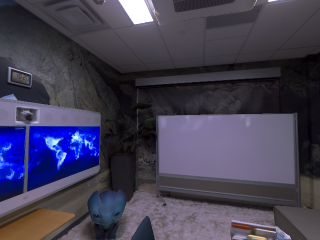
\includegraphics[width=\tw cm,height=\th cm]{keyframe_rgb.png}};
\draw[frm] (rgb.south west) rectangle (rgb.north east);
\node[img, anchor=north] (pca) at (\xA+\wA/2, -2.52) {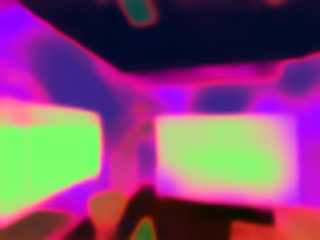
\includegraphics[width=\tw cm,height=\th cm]{features_pca.png}};
\draw[frm] (pca.south west) rectangle (pca.north east);
\draw[arr, black!70] (rgb.south) -- (pca.north) node[midway, right=1pt, lbl] {LSeg};
\node[lbl, anchor=south west, fill=white, fill opacity=0.8, text opacity=1, inner sep=1.2pt]
  at (rgb.south west) {RGB(-D)};

% ================================================================== (2) lifting: one render + one backward
\begin{scope}[shift={(\xB+0.42, -1.55)}]
  % camera
  \draw[black!75, line width=0.5pt, fill=white] (-0.16,-0.20) rectangle (0.10,0.20);
  \draw[black!75, line width=0.5pt, fill=black!10] (0.10,-0.12) -- (0.32,-0.32) -- (0.32,0.32) -- (0.10,0.12) -- cycle;
  % rays to the Gaussians
  \foreach \yy in {0.55,0.05,-0.50}
    \draw[evid!55, line width=0.4pt, dash pattern=on 1.2pt off 1pt] (0.32,0) -- (1.55,\yy);
  % Gaussians (schematic), one highlighted
  \draw[fill=black!12, draw=black!40, line width=0.3pt, rotate around={30:(1.95,0.62)}]  (1.95,0.62) ellipse (0.34 and 0.13);
  \draw[fill=black!12, draw=black!40, line width=0.3pt, rotate around={-25:(2.05,-0.55)}] (2.05,-0.55) ellipse (0.30 and 0.12);
  \draw[fill=black!12, draw=black!40, line width=0.3pt, rotate around={70:(1.55,-0.10)}] (1.55,-0.10) ellipse (0.26 and 0.10);
  \draw[fill=evid!45, draw=evid!80!black, line width=0.45pt, rotate around={-10:(1.92,0.05)}] (1.92,0.05) ellipse (0.36 and 0.15);
\end{scope}
\node[lbl] at (\xB+\wB/2, -2.80) {one render $+$\\ one backward pass};
\node[lbl, text=evidtxt] at (\xB+\wB/2, -3.42) {$\uv_v=\R_v/m_v$,\ \ $\omega_v$};
\node[lbl, text=evidtxt] at (\xB+\wB/2, -3.82) {per Gaussian and view};

% ================================================================== (3) change test, reset, re-admission
\def\cw{2.90} \def\ch{2.175}           % 4:3
\node[img, anchor=north] (chg) at (\xC+\wC/2, -0.52) {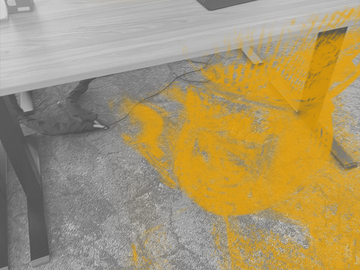
\includegraphics[width=\cw cm,height=\ch cm]{change_nor002.png}};
\draw[frm] (chg.south west) rectangle (chg.north east);
\node[img, anchor=north west, draw=white, line width=0.8pt] (bef) at ($(chg.north west)+(0.06,-0.06)$)
  {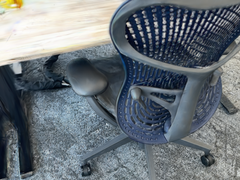
\includegraphics[width=0.95cm,height=0.7125cm]{change_nor002_before.png}};
\node[lbl, anchor=south west, text=white, fill=black, fill opacity=0.55, text opacity=1, inner sep=0.8pt] at (bef.south west) {before};
\node[lbl] at (\xC+\wC/2, -2.98) {$c=1-\cos(\R^{\mathrm{old}},\R^{\mathrm{new}})$};
\node[lbl] at (\xC+\wC/2, -3.38) {$\bar c>\theta(h)$: reset};
\node[lbl, text=chgtxt] at (\xC+\wC/2, -3.84) {re-admitted when\\ the depth agrees};

% ================================================================== (4) running sums -> two uncertainties
\node[draw=evid, fill=white, rounded corners=5pt, inner sep=2.5pt, line width=0.5pt] (sums)
  at (\xD+\wD/2, -0.80) {running sums\ \ $\R,\ W_1,\ W_2,\ Q$};
\def\uw{2.15} \def\uh{1.6125}          % 4:3
\node[img, anchor=north west] (ue) at (\xD+0.20, -1.42) {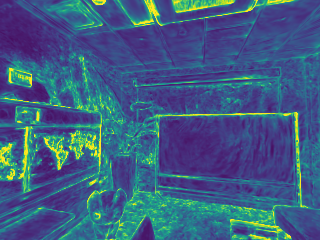
\includegraphics[width=\uw cm,height=\uh cm]{u_epi.png}};
\draw[frm] (ue.south west) rectangle (ue.north east);
\node[img, anchor=north west] (ua) at (\xD+0.20+\uw+0.20, -1.42) {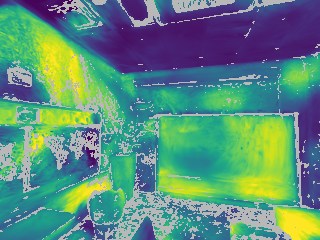
\includegraphics[width=\uw cm,height=\uh cm]{u_ale.png}};
\draw[frm] (ua.south west) rectangle (ua.north east);
\draw[arr, evid] (sums.south) ++(-0.25,0) -- (ue.north);
\draw[arr, evid] (sums.south) ++(0.25,0) -- (ua.north);
\node[lbl, anchor=north] at (ue.south) {$u^{\mathrm{epi}}=\tfrac{1}{1+W_1}$\\[1pt] how much evidence};
\node[lbl, anchor=north] at (ua.south) {$u^{\mathrm{ale}}=1-\hat\rho$\\[1pt] do the views agree};

% ================================================================== (5) text query -> labels
\node[lbl, draw=rd, fill=white, rounded corners=5pt, inner sep=2.5pt, line width=0.5pt] (q)
  at (\xE+\wE/2, -0.80) {text queries $\tv_c$};
\def\lw{1.95} \def\lh{1.4625}          % 4:3
\node[img, anchor=north] (lab) at (\xE+\wE/2, -1.42) {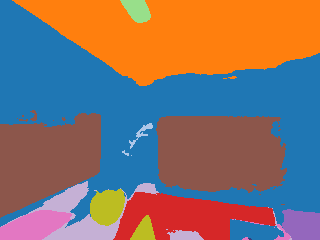
\includegraphics[width=\lw cm,height=\lh cm]{labels_p2.png}};
\draw[frm] (lab.south west) rectangle (lab.north east);
\draw[arr, rd] (q.south) -- (lab.north);
\node[lbl, anchor=north] at (lab.south) {$P(y_p{=}c)\propto$\\[1pt] $\exp(\beta\,\Fv_p^{\!\top}\tv_c)$};

% ================================================================== flow arrows
\draw[arr, black!75] (\xA+\wA, \ymid) -- (\xB, \ymid);
\draw[arr, black!75] (\xB+\wB, \ymid) -- (\xC, \ymid);
\draw[arr, black!75] (\xC+\wC, \ymid) -- (\xD, \ymid);
% the test reads the Gaussian's earlier evidence (the sums before this view)
\draw[arr, chg, dash pattern=on 2.2pt off 1.4pt] (\xD+0.55, -\h) -- (\xD+0.55, -\h-0.30)
  -- (\xC+\wC/2, -\h-0.30) node[pos=0.5, below, lbl, text=chgtxt, inner sep=1.5pt] {earlier evidence of each Gaussian}
  -- (\xC+\wC/2, -\h);
\draw[arr, black!75] (\xD+\wD, \ymid) -- (\xE, \ymid);
% next keyframe
\draw[arr, black!55, dash pattern=on 2.2pt off 1.4pt] (\xD+\wD-0.30, \ytop) -- (\xD+\wD-0.30, 0.38)
  -- (\xA+\wA-0.35, 0.38) node[pos=0.5, above, lbl, text=black!70, inner sep=1pt] {next keyframe}
  -- (\xA+\wA-0.35, \ytop);
\end{tikzpicture}
\end{document}
